%% LyX 2.0.2 created this file.  For more info, see http://www.lyx.org/.
%% Do not edit unless you really know what you are doing.
\documentclass[a4paper,english]{article}
\usepackage[T1]{fontenc}
\usepackage[utf8]{inputenc}
\usepackage{listings}
\setlength{\parskip}{\medskipamount}
\setlength{\parindent}{0pt}
\usepackage{float}
\usepackage{url}
\usepackage{graphicx}

\makeatletter

%%%%%%%%%%%%%%%%%%%%%%%%%%%%%% LyX specific LaTeX commands.
\special{papersize=\the\paperwidth,\the\paperheight}

%% Because html converters don't know tabularnewline
\providecommand{\tabularnewline}{\\}

\makeatother

\usepackage{babel}
\begin{document}

\title{Upgrades as a Service}


\author{Eetu Korhonen, \url{eeko@iki.fi}}


\date{\today}

\maketitle
\url{http://eeko.iki.fi/}

\url{http://github.com/Eeko/mediawiki_uaas/}
\begin{abstract}
This report examines several concepts of performing upgrades for real-time
service applications without usage downtime. This is done by leveraging
some possibilities of using on-demand computing resources provided
by Infrastructure as a Service -providers. Common example of such
application could be a public web-service requiring high availability
for user, yet utilizing centrally maintained server architechture
for operation. 

Within the study we produced a feature-limited prototype of a a tool
intended for providing a live-upgrade from MediaWiki 1.4 to 1.5. The
upgrade originally required over 22 hours of write-lock to the system
when it was applied to the English Wikipedia in 2005. In addition
of building the tool, we explored a set of possible approaches to
help with the upgrade availability problem and the innate challenges
withtheir implementation and use.
\end{abstract}

\section{Introduction}

This document is the end report for an independent research project
performed for EURECOM%
\footnote{\url{http://www.eurecom.fr/}%
} Semester Project -course. The study was done between July 2011 -
January 2012. The purpose of the project was to research and demonstrate
possibilities to leverage flexible cloud-infrastructure to provide
online service updates with very little or no downtime for the end-user.
The project was directed by Dr. Tudor Dumitras from Symantec Research
Labs and supervised by Prof. Marc Dacier from EURECOM.

In the study, we first define the problem of performing service upgrades
without downtime and introduce the concept of using on-demand computing
resources in order to provide flexible capability. This allows us
to trade system downtime into temporary increase in computing resources.
We also examine the case of Wikipedia 1.4 to 1.5 upgrade in 2005,
where the significant table-restructuring originally required a 22
hour write-lock in operations when done for the full Wikipedia dataset.

For this problem, we present a prototype for a software capable of
handling a small subproblem of the said upgrade without requiring
a write-lock in the original database. Namely we present a program
which translates an article upgrade in the old 1.4 schema into the
new 1.5 schema running simultaneously in a replicated computing environment.
The implementation showed a number of limitations, such as the requirement
for translating much of the application logic to a format understandable
by the translator and the need for separate reasoning and decision
logic due to the limited information in the data sources.

After describing the software created, we examine some of the alternate
approaches explored during the project and the issues encountered
with them. Much of the focus with these approaches are beyond just
upgrading an individual application (MediaWiki), but in finding generalizations
and why they might be infeasible for larger, more complex and robust
programs.


\section{Problem}

The high level issue under research is the possibility of performing
system-updates in scale without affecting the availability of service
to the end-user. With system updates changing the functionality of
software, the common case requires an unavailability for the period
while modifications to the system are made. For this study, we reviewed
the Wikipedia upgrade 1.5 from 2005, which required a 22 hour write
lock due to a significant database-schema change, requiring a re-write
of the entire article database.%
\footnote{\url{http://meta.wikimedia.org/wiki/MediaWiki_1.5_upgrade}%
}

There are two conventional methods to avoid availability breaks in
a distributed system. One is to perform the upgrade as a switch-over
where the system is split in two halves. First part of the system
gets upgraded while the other part serves the clients. When the update
is completed, the updated system is switched to be the client-serving
end and the other part applies the same update in turn. This means
the end-user performance of the system is halved during the upgrade.
The second way is to perform the upgrade as a ``rolling wave''.
In Rolling Wave the upgrade is applied to individual nodes of the
distributed system in successive order. This allows for a greater
accuracy in failure localization and reduces risks of failures as
the entire system (or significant parts of it) do not get compromised
for upgrade-errors.

However, neither of these approaches allow a downtimeless upgrade
if the upgrade causes backwards incompatibilities. Any updates into
the non-updated systems should reflect into the updated system as
well. In this study, such incompatibility appears with the database-schema
change of MediaWiki 1.5.


\subsection{Leveraging elastic computing resources for updates}

The examined method of avoiding the incompatibility issues with downtimeless
upgrade is to use external computing resources to clone the existing
service into a ``parallel universe''. In the parallel universe,
the upgrade can be applied without touching the existing system still
providing service to the clients. When the upgrade is successfully
applied into a server cloned from a corresponding existing resource,
the parallel system performs a ``catch-up'' with the changes inserted
into the original client-serving server and starts routing the client
requests into itself. \cite{DBLP:conf/middleware/DumitrasN09a}

Modern cloud computing infrastructures provide us with a platform
for creating and utilizing external resources as needed. Applications
running within Infrastructure as a Service (IaaS) providers such as
Amazon EC2, Rackspace Cloud Servers or OpenNebula are by default running
on virtualized hardware and are generally easily replicable without
large and permanent investments in hardware.


\subsection{MediaWiki 1.4 to 1.5 upgrade}

The June 2005 update to MediaWiki 1.5 was introduced primarily to
perform the schema change examined in this project. Few of the new
features, such as logging the page-rename history and revised permalinking
are dependant on the new schema. But those features do not interfere
with online-upgrading, since the relevant tables can be re-generated
separately from the existing database if needed.

In the 1.4 version of the schema, individual articles contained entries
in two tables. The ``cur''-table contained the most recent revisions
of the articles. The ``old''-table contained the corresponding article
history, usually listing up several related (old wikipage revisions)
entries for a single article in cur-table. The entries in the tables
are connected by the cur-table unique id of ``cur\_namespace + cur\_title''.
A completely new article appears as a new insertion into the cur-table
and a modification creates a new entry to the old-table to where the
contents of the obsolete cur-entry are copied before it gets updated.

In the 1.5 version, the architecture is split into three tables. The
new ``revision'' table is formed by combining the previous old-
and cur-tables and is intended to represent the relevant metadata
for all article insertions and updates of the system - such as the
data of the user who edited the page, the relevant timestamps and
comments of the new update. A revision-entry is connected to a relevant
entry in ``text''-table, which contain the articles themselves.
An entry in revisions also connect to an entry in the ``page''-table,
which represents an individual article with a revision-history in
the revision-table. The most current article is stored in the ``page\_latest''
pointer towards a singular entry in revision-table.

\begin{figure}[H]
\begin{centering}
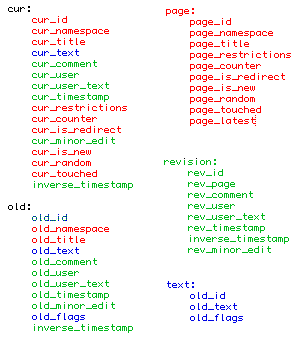
\includegraphics{Database-restructure}
\par\end{centering}

\caption{Database Schema Changes in MediaWiki 1.5 \cite{wiki:SchemaChangeChart} }
\end{figure}



\section{Solution}

We built a small prototype of a software-stack capable of reading
the MySQL query logs in real time from the system providing service
to the end-user. Whenever it detects an update to the article tables
under update, it would create a translation of those queries compatible
with the new schema. After the standard, non-modified, 1.4 to 1.5
update is applied to the parallel universe clone of the system, we
use an external program hooking into the new database. This program
uses the recorded modifications to mimic inserting article updates
to the updated database. When the system under update has reached
a synchronous state with the live-system, we can shut down the old
system, the upgrade programs - and route all traffic to the updated
system.


\subsection{Implementation details}

The original test-system under study is a small-sized%
\footnote{\url{http://aws.amazon.com/ec2/instance-types/}%
} Amazon EC2-instance running a software stack%
\footnote{Amazon Linux 2011.2 with PHP 5.2, Apache 2 and MySQL 5.1 %
} capable of running MediaWiki 1.4 with a custom test-database for
a set of test articles. 


\subsubsection{System replication tools}

To automate the system replication procedure, we developed a series
of bash-scripts leveraging the Amazon EC2-tools and knowledge of the
details of the system under upgrade. Primarily we require the Amazon
instance running details (instance number, public hostname) and the
application information (database name, host, username and password)
for running the replication stack. The system is designed so that
we can use an external node with ssh- and EC2-tools configured to
access to the Amazon control services to download the necessary programs
from repositories and start performing the upgrade process centrally.
Without touching the running instance still providing service for
the clients.

\medskip{}
The main scripts to initiate the upgrading process are as follows:
\begin{itemize}
\item configs.conf -- A sourcable configuration file to set the required
environmental variables in the bash-scripts. Requires manual modifications
to point to the EC2-node to be replicated and to know how to hook
into the database.
\item prepare\_for\_cloning.sh%
\footnote{Not implemented yet as of \today.%
} -- Intended for installing a necessary stack of software to the node
to be replicated. Such as Python 2.7 and mysql-python required by
the updater software. Should also ensure that the required program-versions
are available for the updating scripts in the locations specified
in them.
\item create\_aws\_replica.sh -- Initiates the cloning process by copying
the targeted node disk-image into an Amazon AMI%
\footnote{Requiring a brief shutdown of the said instance.%
} and starting a new identical instance with the said image. Creates
a modified configs.replica -file to include the necessary instance
details needed by the rest of the scripts.
\item setup\_replica.sh -- Copies the necessary scripts and programs into
the new instance via scp.
\item start\_update.sh -- Makes some necessary database-access modifications
into the query-translating programs and starts an SSH-pipe into the
original MediaWiki 1.4 node to stream the query log. This is to be
run in the new, replicated instance.
\item std\_update\_mwiki14-15.sh -- This script contains tools for running
the standard upgrade-procedure to create a new copy of MediaWiki 1.5
running on top of the restructured database. This is to be run in
the new, replicated instance and requires superuser access for the
necessary Apache configuration and reboots. The script downloads MediaWiki
1.5 from the SVN-repository.
\end{itemize}

\subsubsection{Query parser, translator and mapper}

The rest of the software is a series of python-programs used by update\_mediawiki.py.
Update\_mediawiki.py requires an argument of the path to the file
where the original systems query-log has been streamed. It eventually
rewrites all updates detected in existing articles with the new database
schema within the parallel universe.

\medskip{}


The program components are as follows:
\begin{itemize}
\item update\_mediawiki.py -- The entry-point of the program. Contains a
main() method executing the translator-program from translator.py.
\item translator.py -- Contains the logic needed to use the query-log parser
program (parser.py), how to interpret its returns and to translate
them into SQL-queries writable by the database-hookup component. (mysql\-connect.py)
\item parser.py -- Contains the logic required to detect and parse relevant
INSERT and UPDATE queries from MySQL query-logs. The lines we wish
to detect are the ones making article-updating modifications into
an original MediaWiki 1.4 database.
\item mysql\_connect.py -- Helper methods used to interact with a MySQL
database.
\end{itemize}
Developing the software stack from scratch in its current form took
from a single pre-intermediate programmer approximately 80 hours of
research and development time. Though it is to be noted that most
of the time was spent in getting familiar with the less understood
portions of the toolset and the system undergoing the upgrade. Most
of the time allocated for this project (totalling to approximately
250 hours) was spent exploring the problem and the alternate described
approaches for it.

I estimate that doing a similar deployment with full feature set within
similarly limited application could be done in less than 300 hours
with distributed work and decent professionals. Much of the labour
required would be testing work of other use-cases and developing rules
for the architecture to parse. Most of my proof-of-concept programming
were about the necessary infrastructure in parsing relevant queries
and working the communication between the systems. The non-implemented
individual translations and query-detection tools can benefit from
a robust infrastructure, reducing the amount of programming work in
the end parts. Much of the labour could also substitute work needed
to do the regular upgrade. The standard upgrading schema could be
made to utilize translation rules compatible with the real-time updating
procedure. For example, one could substitute the PHP- and SQL-scripts
of the MediaWiki 1.5 upgrade with generalized build tools capable
of rendering the sql-scripts but to also to create the translation
rules for online-upgrade.


\subsection{Problems with the implementation}


\subsubsection{Case-specific}

Our query-detector and translator approach requires us to understand
and re-implement large portions of the application logic within an
external framework. This calls for a significant amount of manual
labor and would intuitively be more suitable to be integrated directly
into the standard upgrading mechanisms rather than providing an external
framework. More notably, individual upgrade-instructions are not recyclable
for other upgrades; neither can we leverage the existing SQL-upgrade
instructions to automate the logic-programming.


\subsubsection{Query-logs as a data source}

Another issue are in the limits of the data extractable from the query
logs. Much of the details ending up to the database can be programmed
and computed to be performed by the database itself without necessarily
revealing them in the query logs E.g. generating entries via database-triggers
and the auto-incrementations of id's are sometimes done within the
database and can't be read from default query-logs. In the lower levels
- the database may perform optimizations or transaction aborts not
necessarily visible to the logs. Or they can be insufficiently hard
to predict and react for in large scale parsing. For adequate understanding
of the workings of the database, the visible plain-text query-logs
are likely insufficient. The approach would be more suited to be done
by using the existing database replication infrastructures and binary-logs,
which reliably reveal the internal database-actions in detail. Though
this is not guaranteed, since the binary logs might omit necessary
data such as the detailed lists of rows affected by a query.


\subsubsection{Inefficiency and fault tolerance}

The implementation looks into the updates as individual transaction,
which is necessary as the program simulates a working application
performing similar actions in a live use scenario. This is hardly
efficient for larger data sets and error prone; should there be unexpected
modifications (such as manual inserts) to the database not detectable
by the developed application. 

Another way would be to use the query-logs to create records of data
requiring action after a stage of upgrade has been completed. For
example, two updates to the same article could be marked as a single
entry to a table of ``touched'' article-id's. Then we make a external
query to the original database to stream the necessary changes into
the parallel universe. This does not free us from implementing some
application logic, as actions like deleting rows or modifying their
unique id's would have to be represented in the tracking logic of
tainted-entries. Neither is it granted that the query-logs available
present us with enough data to identify the tainted items. For example,
an INSERT-query might enter their unique id as NULL and auto-increment
it in the database or application-logic. Such incrementation based
on the MAX(ID)-value of the new flattened text-table of MediaWiki
1.5 was required in our implementation.

Though due to the elasticity of computing resources and low cost of
upgrade-failures, failed upgrades can be tried again as often as needed.
This opens us for possibilities of performing a less-refined probabilistic
upgrade, where we only need a chance for individual upgrade to succeed
and a number of computers performing the upgrade. After a unit passes
tests for schema-equivalence, one can use standard database-replication
suites to duplicate the relevant infrastructure to match the existing
system.


\subsubsection{Limitations of virtualization technology}

It is necessary to note that the current implementation does not manage
fully without downtime, since creating an identical real-time duplicate
in Amazon EC2 requires a downtime to make a copy of the image. However,
it should be possible to make relevant replications in virtualized
production environments, since equivalent copies of the database can
be made without shutting down by using the standard redundancy replication
procedures provided by every major RDBMS. If this is not possible
the shutdowns can be made as a rolling wave, requiring only a minimal
amount of service degration in a horizontally scaled environment.


\section{Alternate approaches}

During the course of the study, several other methods of performing
the online-upgrade were speculated of and experimented with.


\subsection{Using existing database-replication}

One approach we experimented with was trying to leverage an existing
database-reflection infrastructure. Namely, the GORDA%
\footnote{GORDA Open Replication of DAtabases%
}%
\footnote{\url{http://gorda.di.uminho.pt/}%
} database replication architecture. GORDA is a set of extensions for
a range of RDBMS's offering an external API-access and for the inner
workings of the databases. Most common RDBMS's offer a number of reflective
interfaces, such as the used query-logger and described binary-loggers
-- but they often fall short with certain atomicity features in distributed
setups.%
\footnote{Such as the visibility of commit-order and capabilities to view and
influence the client commits.%
} \cite{Carvalho_onthe}

GORDA would help us by providing us the necessary infrastructure for
reflecting the database interactions %
\footnote{Which was done by the query-parser of our implementation.%
} and it would provide a programmable interface capable of instructing
the parallel database.%
\footnote{Done in the translator and connector classes of our solution.%
} This would all be done within the extended databases where the atomicity
and reflection-reliability issues would be handled by GORDA. \cite{DBLP:dblp_conf/nca/CorreiaPRCVOG07}

However, there proved to be a number of issues with this approach.
Firstly, the most mature implementation of GORDA compatible with MediaWiki
was one hooking up into a PostgreSQL database. For MediaWiki 1.4,
the PostgreSQL -support was considered to be ``experimental'' and
it was recommended to use MySQL for production database. After the
schema upgrade in 1.5, the PostgreSQL-support was officially discarded,
though the unmodified components were still within the source code.
Making the software run on PostgreSQL (or Apache Derby, which is ``default''
database for GORDA) requires a number of extra modifications.

Secondly, GORDA itself is still on a prototype stage. Orienting into
it and extending it to fit the system at stake proved to be infeasible
within the scope and skill level involved with the project. The most
time-consuming issues being that the current prototype showed to lack
support for a number of features%
\footnote{Such as namespace support in table naming.%
} and necessary documentation. This project did not manage to examine
the GORDA system enough to give estimates on the difficulty and time
requirements for continuing with the approach. Some issues figured
out could be circumvented by reconfiguring the application but at
the stage of abandoning the approach%
\footnote{After approximately 120 hours of development.%
} - the risk probability and time required for additional unknown obstacles
were considered too high.


\subsection{Using similarity in application calls}

Another idea to provide upgrades as a service for an ongoing database
upgrade would be to move the upgrade-synchronization away from the
database-layer. If an upgrade touches only the underlying database
layer and the application interface connecting to it, one could cache
and re-route identical application calls to a parallel-universe backend
replicating similar functionality within different schema. This kind
of upgrade would naturally suit a typical 3-tiered web-application,
where the user transactions provided by web-server are separated from
a dynamic content engine and data storages.

\begin{figure}[H]
\begin{centering}
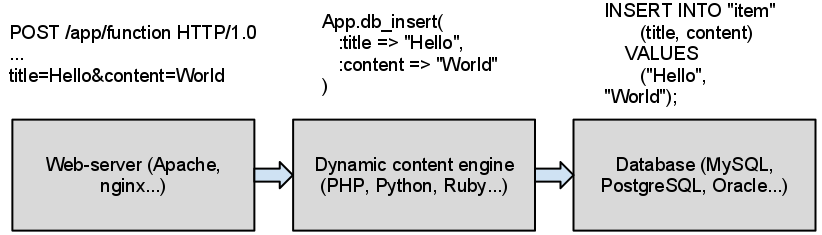
\includegraphics[width=1\columnwidth]{3-tier}\caption{A typical 3-tiered web application}

\par\end{centering}

\end{figure}


Should the interface to the frontend-engine stay identical, this kind
of approach would provide an easy and elegant solution for making
a seamless transition to new software version without requiring any
adaptations or query mappings between the systems. In the case of
MediaWiki 1.4 to 1.5 upgrade, the main focus of the upgrade was this
database-schema change. The upgrade could have been split into parts
only affecting the application \& database layers while keeping the
user facing web server interface the same. Should an upgrade provide
any UI modifications, those could be made in an another upgrade-package
keeping the database untouched.

\begin{figure}[H]
\begin{centering}
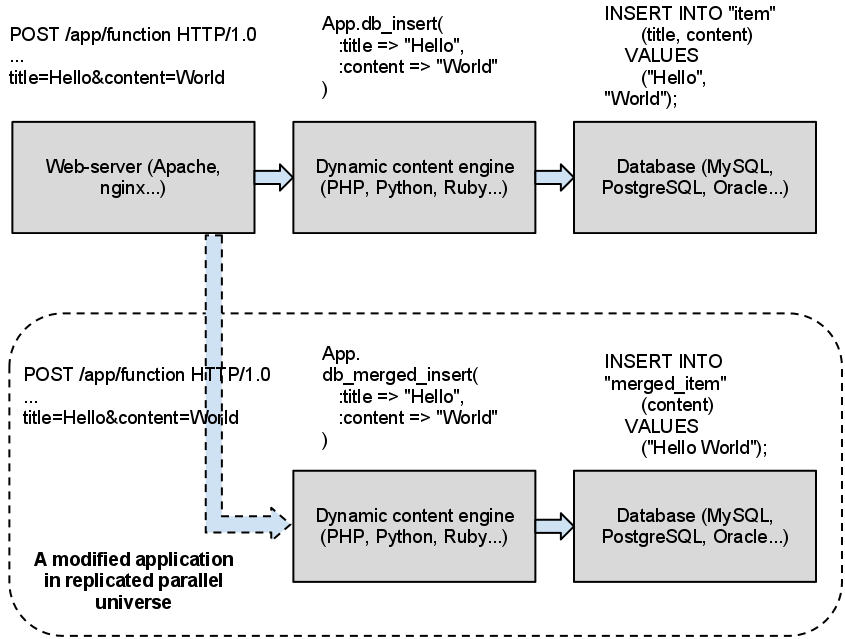
\includegraphics[width=1\columnwidth]{3-tierinparallel}\caption{A 3-tiered web application routing interface-queries to original and
upgraded backends}

\par\end{centering}

\end{figure}


Not every kind of software update would work with this approach. Several
upgrades implement new functionality with a need for wide modifications
to every layer of the software. Though often such upgrades can be
split into incremental parts where the heavy database-modifying and
writing operations can be done before the corresponding modifications
are introduced to the frontend. As this requires additional engineering-consideration
for upgradeability, it might not be feasible to provide upgrading
as an external service for application-upgrades modifying the entire
stack.

Other issue would be the lack of guarantees for consistency in the
entire stack. Should there be failures in the middle- or database-tier
of the live system, a dumb frontend-replicator would not detect them
nor present adequate information to account the inconsistency in the
parallel universe. Such issues could be coped with most standard redundancy
\& reliability techniques utilized in the system. The redundancy technology
can be made to monitor and require confirmation of commits from the
backend or from redundancy replication interfaces. Or with cheap replicable
virtual hardware, we could settle with eventual consistency where
we just restart an upgrade-procedure until the backend passes sufficient
tests of equivalence.

\begin{figure}[H]
\begin{centering}
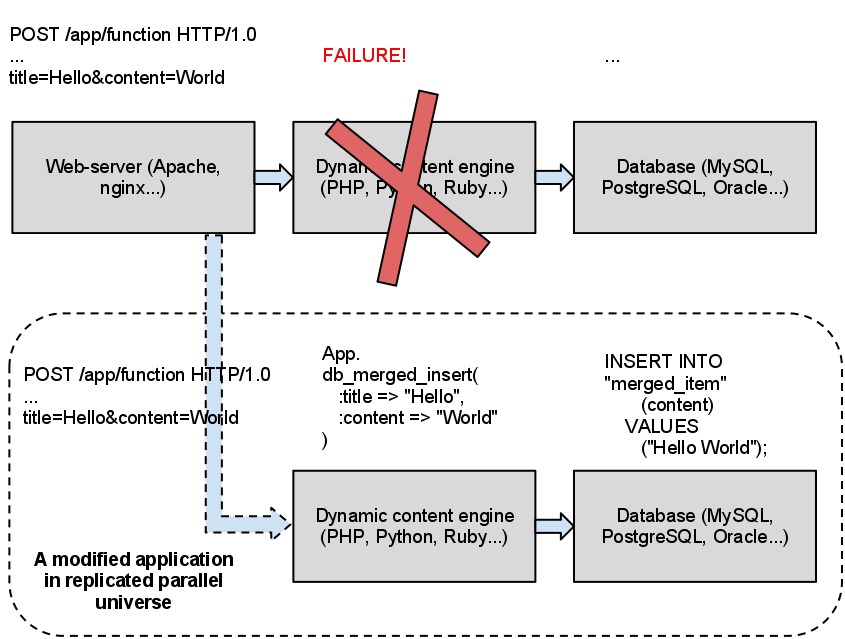
\includegraphics[width=1\columnwidth]{3-tierinparallelfailure}\caption{A faulty parallel-run leaving the two systems in inequivalent states}

\par\end{centering}

\end{figure}



\subsection{Using the existing upgrade tools to decreasing database subsets}

One of the more intriguing approaches would be to create a framework
capable of reading the existing schema-upgrade scripts available and
deduct the upgrade logic and resulting tables from them. Since the
target tables are expanding leading to increasing time-requirements
of re-applying the updates to complete tables, we need to be able
to divide the work into smaller subsets as new items and updates get
inserted during the online-upgrade.

An intuitive way for such division would be to split the dataset under
update by their timestamps, so that we only re-run the standard upgrade
script for new items inserted after the last known item in the databases
under upgrade was received. However, under some upgrades this will
lead to different results than a normal, singular update and possibly
broken consistency due to the unpredictability of the live-system
updates.

\medskip{}


MediaWiki 1.4 used two separate tables to represent articles (cur-table)
and their revision history (old-table). The tables contain mostly
similar information allowing the history to be formed by copying the
old contents of cur-table to be archived in old-table. The upgrade
in MediaWiki 1.5 system combines these and splits them into three
tables containing different logical fractions of the data.

In our example, we have generalized the first combining operation
into a higher abstraction of state-entries (``cur'', as in MediaWiki
1.4) and history-entries (``old'', as in MediaWiki 1.4). Every history
entry has a foreign key pointer to a corresponding current state.
Performing incremental joins within this kind of database leads into
an inconsistent state compared to a singular batch operation done
with similar joins.

\begin{table}[h]
\centering{}%
\begin{tabular}{|c|c|}
\hline 
cur\_id & cur\_content\tabularnewline
\hline 
\hline 
1 & 1\_Fourth\_state\tabularnewline
\hline 
2 & 2\_Second\_state\tabularnewline
\hline 
\end{tabular}\caption{Current states -table (cur-table)}
\end{table}


\begin{table}[H]
\centering{}%
\begin{tabular}{|c|c|c|}
\hline 
old\_id & old\_content & old\_link\_to\_cur\tabularnewline
\hline 
\hline 
1 & 1\_First\_state & 1\tabularnewline
\hline 
2 & 1\_Second\_state & 1\tabularnewline
\hline 
3 & 2\_First\_state & 2\tabularnewline
\hline 
4 & 1\_Third\_state & 1\tabularnewline
\hline 
\end{tabular}\caption{Old states history -table (old-table)}
\end{table}


Suppose, that a schema upgrade would flatten these said tables into
one table containing both the current state of the items and the given
history of said items. An upgrade would be done with the following
SQL-code:

\inputencoding{latin9}\begin{lstlisting}
-- Note, that the primary id's of the table are
-- auto-incremented.
-- This is similar to how Mediawiki 
-- upgrade handles the database-flatten 
-- operation.
INSERT INTO "old" (old_content, old_link_to_cur) 
	SELECT (cur_content, cur_id)
	FROM "cur";
\end{lstlisting}
\inputencoding{utf8}

After the update, the new table would look like this:

\begin{table}[H]
\centering{}%
\begin{tabular}{|c|c|c|}
\hline 
old\_id & old\_content & old\_link\_to\_cur\tabularnewline
\hline 
\hline 
1 & 1\_First\_state & 1\tabularnewline
\hline 
2 & 1\_Second\_state & 1\tabularnewline
\hline 
3 & 2\_First\_state & 2\tabularnewline
\hline 
4 & 1\_Third\_state & 1\tabularnewline
\hline 
5 & 1\_Fourth\_state & 1\tabularnewline
\hline 
6 & 2\_Second\_state & 2\tabularnewline
\hline 
\end{tabular}\caption{Merged old-table}
\end{table}


Suppose that we receive a third state to the original-system during
the time taken by the upgrade and it receives several updates for
it. We have sufficient translation logic in place to only apply the
INSERT-queries for items entered to the database after we begun merging
our previous entries. The code would work something like this:

\inputencoding{latin9}\begin{lstlisting}
-- We first apply the modifications from old-table
INSERT INTO "old" (old_content, old_link_to_cur)
	SELECT (old_content, old_link_to_cur)
	FROM "olddb.old"
	WHERE timestamp > last_update_time;

-- Then we flatten the items from the table of 
-- current states
INSERT INTO "old" (old_content, old_link_to_cur)
	SELECT (old_content, old_link_to_cur)
	FROM "olddb.cur"
	WHERE timestamp > last_update_time;
\end{lstlisting}
\inputencoding{utf8}

Then when we would receive the following rows into the database:

\begin{table}[H]
\begin{centering}
\begin{tabular}{|c|c|c|}
\hline 
old\_id & old\_content & old\_link\_to\_cur\tabularnewline
\hline 
\hline 
5 & 3\_First\_state & 3\tabularnewline
\hline 
\end{tabular}
\par\end{centering}

\centering{}\caption{New row in old-table inserted during the update}
\end{table}
\begin{table}[H]
\begin{centering}
\begin{tabular}{|c|c|}
\hline 
cur\_id & cur\_content\tabularnewline
\hline 
\hline 
3 & 3\_Second\_state\tabularnewline
\hline 
\end{tabular}
\par\end{centering}

\centering{}\caption{New row in cur-table inserted during the update}
\end{table}


We would end up with a merged table looking like the following:

\begin{table}[H]
\centering{}%
\begin{tabular}{|c|c|c|}
\hline 
old\_id & old\_content & old\_link\_to\_cur\tabularnewline
\hline 
\hline 
1 & 1\_First\_state & 1\tabularnewline
\hline 
2 & 1\_Second\_state & 1\tabularnewline
\hline 
3 & 2\_First\_state & 2\tabularnewline
\hline 
4 & 1\_Third\_state & 1\tabularnewline
\hline 
5 & 1\_Fourth\_state & 1\tabularnewline
\hline 
6 & 2\_Second\_state & 2\tabularnewline
\hline 
7 & 3\_First\_state & 3\tabularnewline
\hline 
8 & 3\_Second\_state & 3\tabularnewline
\hline 
\end{tabular}\caption{Merged old-table after incremental upgrade}
\end{table}


If the upgrade would have been done with write-locks and the two tables
would be merged after all 8 commits were received in the same sequential
order as in our online-example, the resulting table would look like
this:

\begin{table}[H]
\centering{}%
\begin{tabular}{|c|c|c|}
\hline 
old\_id & old\_content & old\_link\_to\_cur\tabularnewline
\hline 
\hline 
1 & 1\_First\_state & 1\tabularnewline
\hline 
2 & 1\_Second\_state & 1\tabularnewline
\hline 
3 & 2\_First\_state & 2\tabularnewline
\hline 
4 & 1\_Third\_state & 1\tabularnewline
\hline 
5 & 3\_First\_state & 3\tabularnewline
\hline 
6 & 1\_Fourth\_state & 1\tabularnewline
\hline 
7 & 2\_Second\_state & 2\tabularnewline
\hline 
8 & 3\_Second\_state & 3\tabularnewline
\hline 
\end{tabular}\caption{Merged-old table without online-upgrading}
\end{table}


The id's for items in the different upgrade-approaches are not equivalent.
If it is used as an external-id in somewhere else in database-logic
without the necessary modifications, we will end in faulty behaviour.
To fix this, we need to implement some amount of application- or database-logic
to upgrade corresponding tables with old\_id references.

This would likely not be a problem within the MediaWiki, since the
id's are supposedly used only for separating primary id's from each
other and the supposed order carries no significance. However, inconsistency
of incrementation might be an issue for some programs. Such as ones
requiring predictable consistency with FETCH FIRST {[}N{]} -queries\cite{iso9075-3}
for (un)ordered data or non-standard SQL such as TOP or LIMIT -syntaxes.


\section{Future work}

Although the approach with GORDA proved to be unfeasible in this scope,
different methods to leverage the reflections from database-internals
to provide upgrades as a service are still to be examined. Other possibilities
to get sufficient data could be to hook up into existing database
replication protocols or into the binary-logs used by the said replication
protocols.

And even if the other introduced methods to perform upgrades externally
in replicated environments are not generazible, we have still to examine
whether they might be sufficient for individual cases such as the
MediaWiki upgrade presented. Especially given the simplicity of rerouting
high-level application calls for replicated cloud-servers, designing
upgrades to support it could prove to be a decent engineering practice
for online-services.

Though this study does not help much with re-trying the GORDA-route,
one could examine the costs of extending the most common database
replication protocols to suit dynamic modifications to the queries
and for presenting more detailed views on the interactions to support
an upgrade-compatible replication procedure.


\section{Conclusions}

The implementation provided falls short with the initial goal of performing
an online upgrade in a scale comparable to a real-life use scenario.
(I.e. the entire Wikipedia and updates performed to it during the
upgrade.) Though we manage to explore several approaches for the task
and the challenges involved. The challenges mostly relate with the
need to model much of the application logic within the mapper and
the unreliabliness of the used data-source. The former would be solvable
by being able to utilize the upgrading schema in a suitable framework
and applications. The latter could be figured out by extending and
reconfiguring the logging protocols themselves.

In addition, we have examined a number of other approaches capable
of providing a non-downtime upgrade-procedure in a replicated system
and shown via contradiction, why some of them would be inadequate
for selected, common database-modifying procedures. Though used as
an initial approach for the upgrade, we were unsuccessful in utilizing
the most promising method of leveraging database-reflection interfaces.

\bibliographystyle{plain}
\bibliography{sources}

\end{document}
